\subsection{Authenticator}

Der \emph{Authenticator} ist eine konkrete Implementierung des \nameref{sec:singleaccesspoint}. Er ermöglicht einem Betriebssystem die Verifizierung der Identität eines bestimmten Benutzers.

Dabei ist die Art und Weise, wie eine Identität verifiziert werden kann flexibel austauschbar.


\subsection*{Kontext}
Ein Betriebssystem prüft beim ersten Anmelden am System (evtl. später erneut) die Identität des Benutzers. Das System erstellt dabei nötige Session Context Informationen. Der Benutzer wird anschliessend durch einen User Process im System abgebildet.

Beim Zugriff auf sensitive Daten kann das System erneut nach einer Authentifizierung verlangen.

Das \emph{Authenticator}-Pattern soll auch auf einem verteilten System eingesetzt werden können.


\subsection*{Problem}
Es gibt Benutzer, welche berechtigt Zugriff auf ein System haben. Wie kann verhindert werden, dass unter Voraussetzung folgender Punkte ein Angreifer sich als ein solcher Benutzer ausgeben kann?

\begin{itemize}
	\item Tendenziell gibt es eine grosse Anzahl an Benutzern, welche evtl. sogar verschiedene/flexible Authentifizierungs-Verfahren benutzen
	\item Benutzer dürfen die Sicherheitsprüfung nicht umgehen können.
	\item Benutzer/Angreifer dürfen das Resultat der Sicherheitsprüfung (Token etc.) nicht zu ihren Zwecken verfremden können (Session Hijacking etc.)
	\item Die potenzielle Komponente ist zentral und wird ziemlich sicher oft und auch wiederholt zum Einsatz kommen. Performance ist darum essentiell.
\end{itemize}


\subsection*{Lösung}
Eine spezifische Implementation des \nameref{sec:singleaccesspoint}, der \emph{Authenticator} übernimmt die Verifizierung der Identität eines Benutzers.

Konnte diese erfolgreich durchgeführt werden, erstellt er einen \emph{Proof of Identity} welcher zu späteren Zeitpunkten wiederholt zur Autorisierung im System verwendet werden kann.

Der \emph{Proof of Identity} dient ebenfalls dazu, um weitere, ``aufbauende'' Sicherheitsüberprüfungen in sensibleren Systembereichen durchzuführen.

\begin{figure}[H]
	\centering
	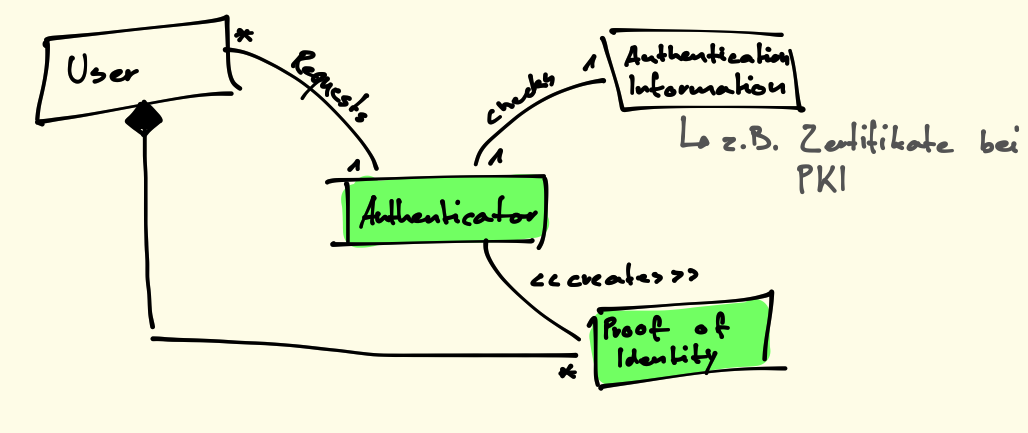
\includegraphics[width=10cm]{content/security/operating-system-access-control/images/authenticator.png}
	\caption{Authenticator: Schematischer Aufbau}
\end{figure}

\subsection*{Vorteile}
\begin{itemize}
	\item Verschiedene Authentifizierungsverfahren können angewendet werden (abhängig von Policies natürlich)
	\item \emph{Authentication Information} wird getrennt vom \emph{Authenticator} gespeichert und verwaltet und kann so explizit geschützt werden. (Readonly etc.)
	\item Durch die Struktur des \emph{Authenticator}-Patterns kann es problemlos in verteilten Systemen angewendet werden.
	\item Die Wiederverwendung des \emph{Proof of Identity} können wiederholende Authentifizierungen vermieden resp. vereinfacht werden
\end{itemize}

\subsection*{Nachteile}
\begin{itemize}
	\item Zeitaufwand
	\item Komplexität und Kosten
\end{itemize}

\subsection*{Reallife Beispiele}
\begin{itemize}
	\item Das aus Enterprise-Netzwerk-Systemen bekannte \emph{Single Sign On} ist eine Variante des \emph{Authenticator}-Patterns.\\
	Der \emph{Proof of Identity} wird da meistens mittels einer PKI generiert und anschliessend von verschiedenen Applikationen zur Identifizierung des Benutzers verwendet, ohne erneut nach den Authentifizierungs-Merkmalen (Passwort, Smartcard etc.) zu fragen.
\end{itemize}

\subsection*{Mögliche Prüfungsfragen}
\begin{itemize}
	\item \emph{Welche Security Patterns sind im Authenticator umgesetzt?}\\
	Der Authenticator ist eine konkrete Implementation des \nameref{sec:singleaccesspoint}-Patterns.
\end{itemize}